\documentclass{beamer}

\mode<presentation> {
% Colors

%\usetheme{default}
%\usetheme{AnnArbor}
%\usetheme{Antibes}
%\usetheme{Bergen}
%\usetheme{Berkeley}
%\usetheme{Berlin}
%\usetheme{Boadilla}
%\usetheme{CambridgeUS}
%\usetheme{Copenhagen}
%\usetheme{Darmstadt}
%\usetheme{Dresden}
%\usetheme{Frankfurt}
%\usetheme{Goettingen}
%\usetheme{Hannover}
\usetheme{Ilmenau}
%\usetheme{JuanLesPins}
%\usetheme{Luebeck}
%\usetheme{Madrid}
%\usetheme{Malmoe}
%\usetheme{Marburg}
%\usetheme{Montpellier}
%\usetheme{PaloAlto}
%\usetheme{Pittsburgh}
%\usetheme{Rochester}
%\usetheme{Singapore}
%\usetheme{Szeged}
%\usetheme{Warsaw}

%Themes

%\usecolortheme{albatross}
%\usecolortheme{beaver}
%\usecolortheme{beetle}
%\usecolortheme{crane}
%\usecolortheme{dolphin}
%\usecolortheme{dove}
%\usecolortheme{fly}
%\usecolortheme{lily}
%\usecolortheme{orchid}
%\usecolortheme{rose}
%\usecolortheme{seagull}
%\usecolortheme{seahorse}
%\usecolortheme{whale}
%\usecolortheme{wolverine}

%\setbeamertemplate{footline} % To remove the footer line in all slides uncomment this line
%\setbeamertemplate{footline}[page number] % To replace the footer line in all slides with a simple slide count uncomment this line

\setbeamertemplate{navigation symbols}{} % To remove the navigation symbols from the bottom of all slides uncomment this line
}

\usepackage{graphicx} % Allows including images
\usepackage{booktabs} % Allows the use of \toprule, \midrule and \bottomrule in tables
\usepackage{tikz}
\usepackage{graphicx}
\usepackage{epstopdf}
\usepackage{amsmath} 
\usetikzlibrary{intersections}
\usetikzlibrary{circuits.ee.IEC}
\usetikzlibrary{calc}
\usetikzlibrary{shapes,arrows}
%----------------------------------------------------------------------------------------
%	TITLE PAGE
%----------------------------------------------------------------------------------------

\title[NMR Assignment with A*]{Accelerating Biomolecular Nuclear Magnetic Resonance Assignment with A*} % The short title appears at the bottom of every slide, the full title is only on the title page

\author[J. Venzke, P. Johnson, R. Davis, J. Emmons, K. Roth, D. Mascharka, L. Robison, T. Urness, A. Kilpatrick]{Joel Venzke, Paxten Johnson, Rachel Davis, John Emmons,\\ Katherine Roth, David Mascharka, Leah Robison,\\ Timothy Urness and Adina Kilpatrick} % Your name
\institute[Drake University] % Your institution as it will appear on the bottom of every slide, may be shorthand to save space
{
Department of Mathematics and Computer Science\\
Drake University\\

\medskip
\textit{joel.venzke@drake.edu} % Your email address
}
\date{April 10,2014} % Date, can be changed to a custom date

\begin{document}

\begin{frame}
\titlepage % Print the title page as the first slide
\end{frame}

% =======================================================================
% =======================================================================
\section{Introduction}
\begin{frame}
\frametitle{Overview} % Table of contents slide, comment this block out to remove it
\tableofcontents 
\end{frame}

\subsection{Motivation} 
\begin{frame}
	\frametitle{Motivation}
	\begin{itemize}
		\item Nuclear Magnetic Resonance Spectroscopy
		\begin{itemize}
			\item Gain knowledge about protein structure
			\item Study how mutations lead to diseases
		\end{itemize}
		\item Problems
		\begin{itemize}
			\item Generates large amounts of data
			\item Data analysis is slow and error prone 
		\end{itemize}
		\item Goal
		\begin{itemize}
			\item Automate the assignment process
			\item Decrease human error
			\item Increase productivity
		\end{itemize}
	\end{itemize}
\end{frame}

% =======================================================================
\subsection{Nuclear Magnetic Resonance Spectroscopy} 
\begin{frame}
	\frametitle{Nuclear Magnetic Resonance (NMR)}
	\begin{itemize}
		\item Used to obtain structural information 
		\begin{itemize}
			\item Chemical shift values
		\end{itemize}
		\item HNCACB experiment
		\begin{itemize}
			\item Generates $C_\alpha$ and $C_{\beta}$ residue $i$ and $i-1$
		\end{itemize}
		\item CBCA(CO) NH experiment 
		\begin{itemize}
			\item Generates $C_\alpha$ and $C_{\beta}$ for residue $i$
			\item Confirms residue data
		\end{itemize}
	\end{itemize}
\end{frame}

\begin{frame}
	\frametitle{Chemical Shift Values}
	\begin{figure}[H]
	\begin{center}
	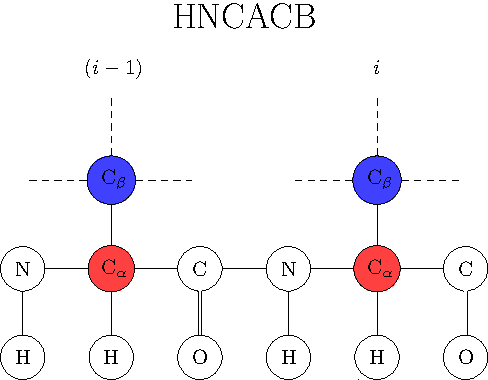
\includegraphics[width=.65\textwidth]{diagram}
	\end{center}
	\end{figure}
\end{frame}



% =======================================================================
% =======================================================================
\section{NMR Assignment Background}

% =======================================================================
\subsection{Data Collection and Manual Assignment}

\begin{frame}
	\frametitle{Manual Methods}
	\begin{itemize}
		\item Most time consuming part
		\item Missing and ambiguous data forces chunks to be skipped
		\item Prone to human error
	\end{itemize}

\end{frame}

\begin{frame}
	\frametitle{Timeline}
	
	\vspace{1.5cm}
	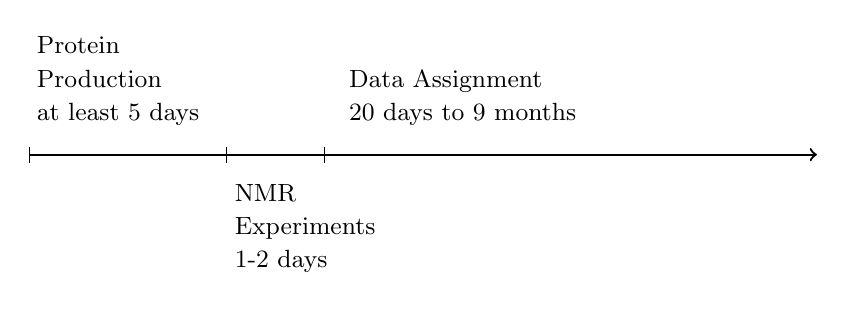
\begin{tikzpicture} [scale=.5]

		\draw [thick, ->] (0,0) -- (20,0);

		\draw (0,-.2) -- (0, .2);

		\draw (5,-.2) -- (5, .2);

		\draw (7.5,-.2) -- (7.5, .2);

		\node[align=left, above] at (2.25,.5)%
		{\small Protein\\ \small Production\\ \small at least 5 days};

		\node[align=left, below] at (7,-.5)%
		{\small NMR\\ \small Experiments\\ \small 1-2 days};

		\node[align=left, above] at (11,.5)%
		{\small Data Assignment\\ \small 20 days to 9 months};
	\end{tikzpicture}

	\vspace{1cm}
	\hfill \scriptsize \cite{babak_alipanahi_error_2011}
\end{frame}



% =======================================================================
% =======================================================================
\section{Automation Algorithm}

% =======================================================================
\subsection{Preprocessing}
\begin{frame}
\frametitle{Automating Assingment}
	\begin{itemize}
		\item Initialization
		\item Generating child nodes
		\item Goal State
		\item Solution State
	\end{itemize}
\end{frame}

\begin{frame}
	\frametitle{Initialization}
	\begin{itemize}
		\item Expected amino acid sequence
		\begin{itemize}
			\item Converted to expected chemical shift values
			\item Stored as the reference protein chain
		\end{itemize}
		\item NMR experiment's chemical shift data
		\begin{itemize}
			\item $C_\alpha$ and $C_{\beta}$ for residue $i$ and $i-1$
			\item Stored in a tile
		\end{itemize}
		\item Missing data
		\begin{itemize}
			\item Place holder tile generation
		\end{itemize}
		\item Grouping 
	\end{itemize}
\end{frame}

\begin{frame}
	\frametitle{Grouping}
	\begin{figure}[H]
	\begin{center}
	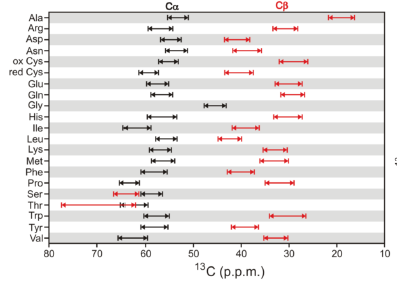
\includegraphics[width=.65\textwidth]{carbon}
	\end{center}
	\end{figure}
\hfill \scriptsize\cite{carbon}
\end{frame}

% =======================================================================
\subsection{Assignment}

\begin{frame}
	\frametitle{Starting the assignment}
	\vspace{-.5cm}
	\center
	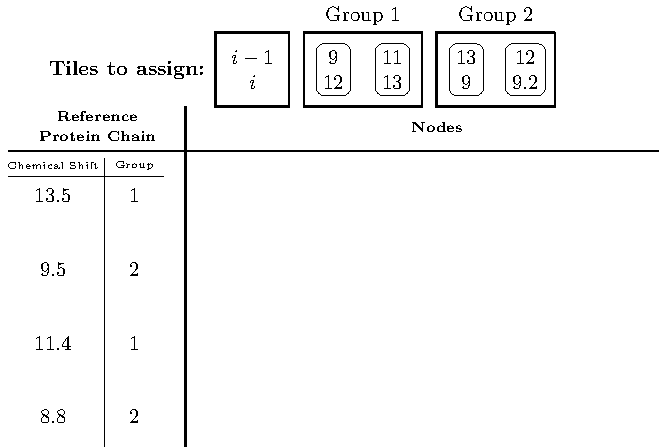
\includegraphics[width=.9\textwidth]{tilePlacement/step1}
\end{frame}

\begin{frame}
	\frametitle{Starting the assignment}
	\vspace{-.5cm}
	\center
	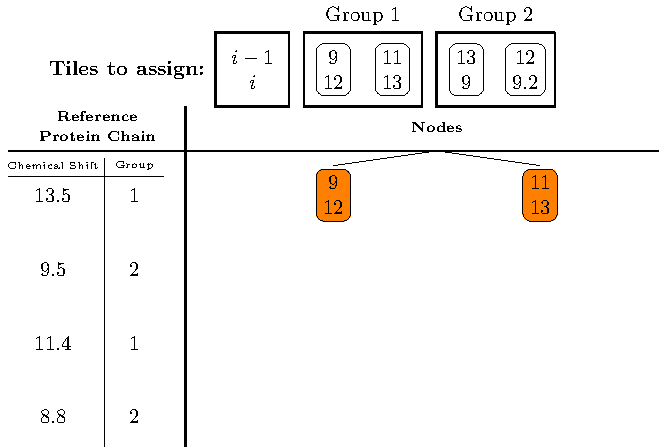
\includegraphics[width=.9\textwidth]{tilePlacement/step2}
\end{frame}

\begin{frame}
	\frametitle{Cost Calculation}
	\begin{itemize}
		\item Accuracy matching the protein chain residue
		\item Accuracy matching the tile above current tile
		\item Cost of placing all previous tiles
	\end{itemize}
\end{frame}

\begin{frame}
	\frametitle{Generating child nodes}
	\vspace{-.5cm}
	\center
	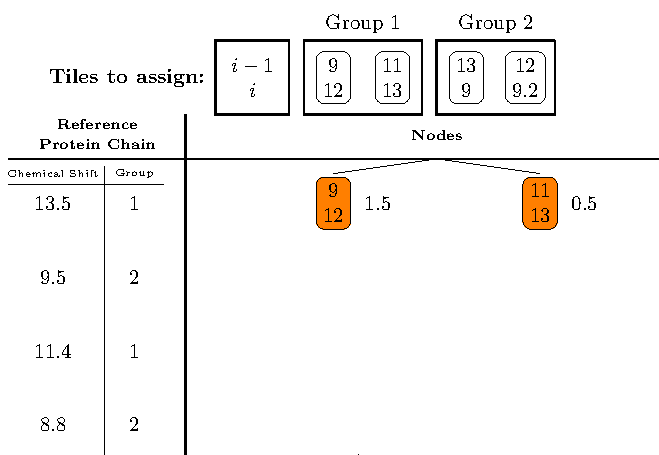
\includegraphics[width=.9\textwidth]{tilePlacement/step3}
\end{frame}

\begin{frame}
	\frametitle{Generating child nodes}
	\vspace{-.5cm}
	\center
	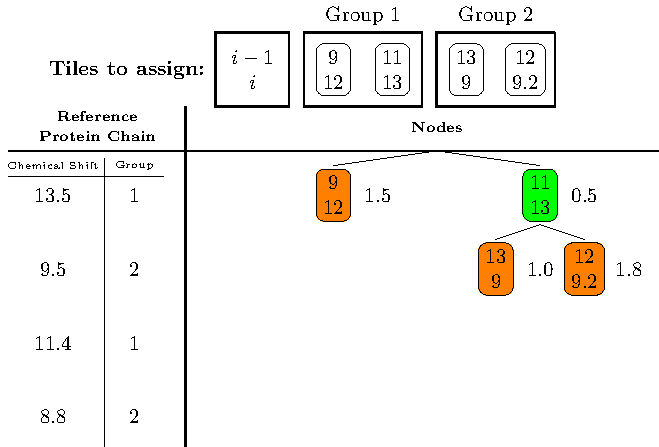
\includegraphics[width=.9\textwidth]{tilePlacement/step4}
\end{frame}

\begin{frame}
	\frametitle{Generating child nodes} 
	\vspace{-.5cm}
	\center
	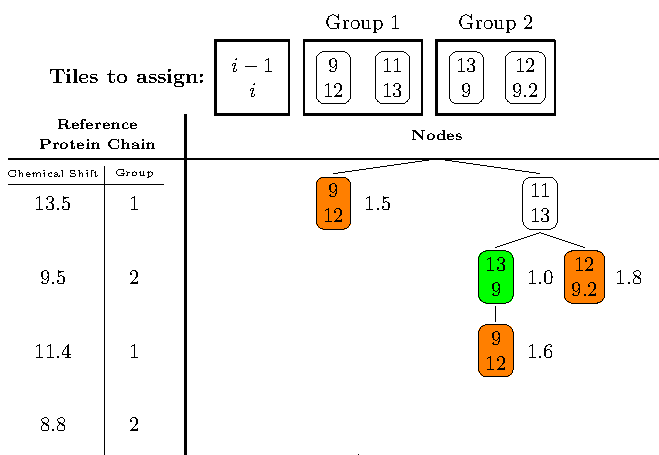
\includegraphics[width=.9\textwidth]{tilePlacement/step5}
\end{frame}

\begin{frame}
	\frametitle{Generating child nodes} 
	\vspace{-.5cm} 
	\center
	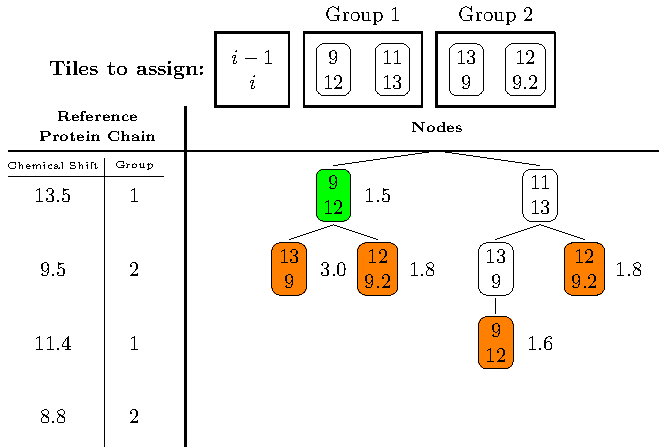
\includegraphics[width=.9\textwidth]{tilePlacement/step6}
\end{frame}

\subsection{Goal State}
\begin{frame}
	\frametitle{Goal State}
	\vspace{-.5cm} 
	\center
	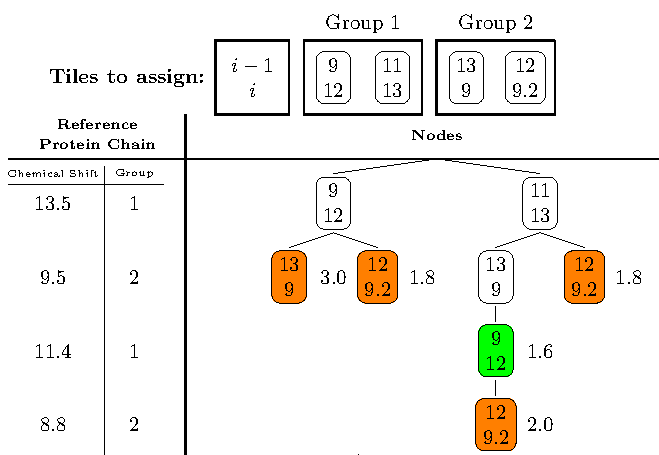
\includegraphics[width=.9\textwidth]{tilePlacement/step7}
\end{frame}

\begin{frame}
	\frametitle{Goal State}
	\vspace{-.5cm} 
	\center
	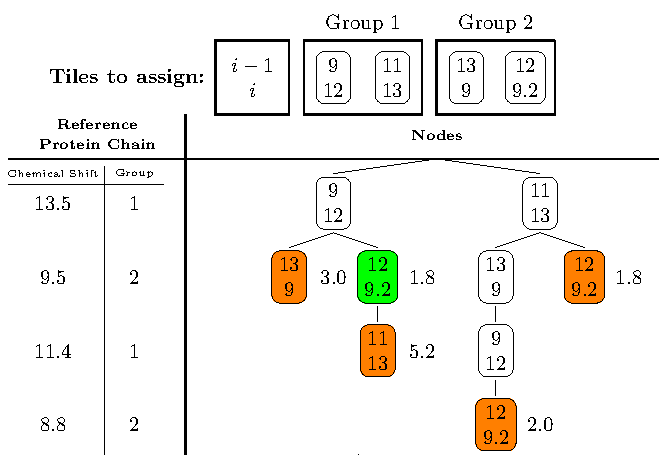
\includegraphics[width=.9\textwidth]{tilePlacement/step8}
\end{frame}

\begin{frame}
	\frametitle{Goal State}
	\vspace{-.5cm} 
	\center
	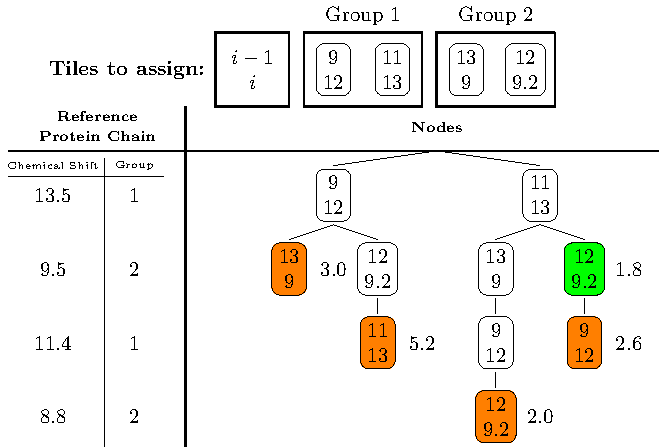
\includegraphics[width=.9\textwidth]{tilePlacement/step9}
\end{frame}

\begin{frame}
	\frametitle{Solution State}
	\vspace{-.5cm} 
	\center
	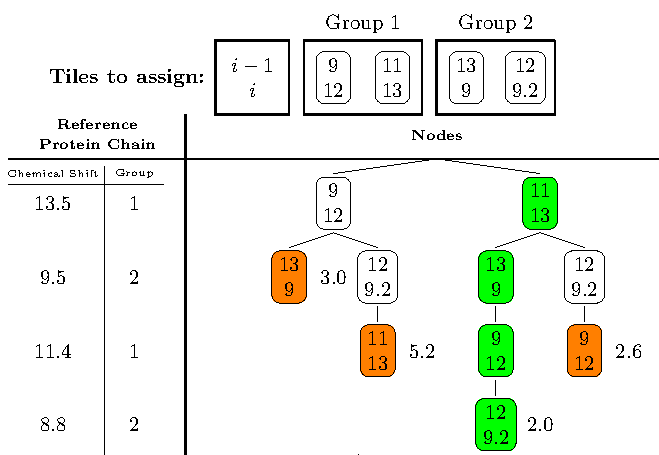
\includegraphics[width=.9\textwidth]{tilePlacement/step10}
\end{frame}

% =======================================================================
% =======================================================================
\section{Conclusion}

% =======================================================================
\subsection{Results}

\begin{frame}
	\frametitle{Time of Assignment}
	\begin{figure}[H]
	\begin{center}
	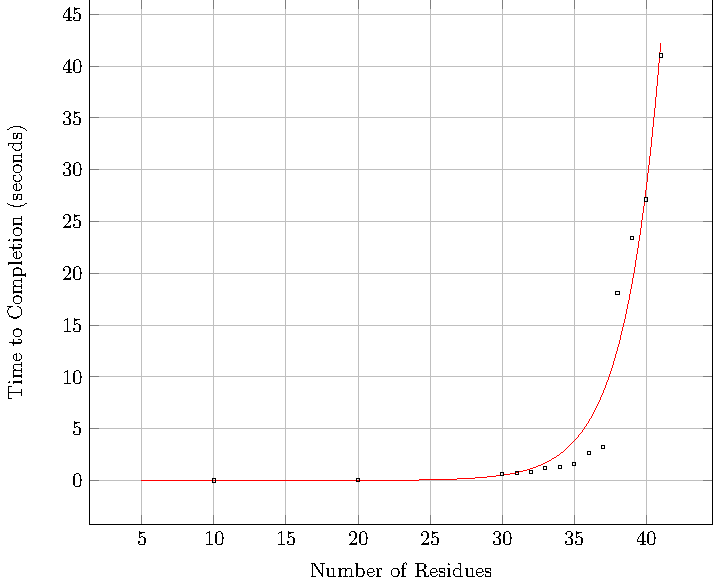
\includegraphics[width=.65\textwidth]{plot}
	\end{center}
	\end{figure}
\end{frame}

\begin{frame}
	\frametitle{Child Nodes Generated}
	\begin{figure}[H]
	\begin{center}
	\resizebox{!}{.6\paperheight}{% GNUPLOT: LaTeX picture with Postscript
\begingroup
  \makeatletter
  \providecommand\color[2][]{%
    \GenericError{(gnuplot) \space\space\space\@spaces}{%
      Package color not loaded in conjunction with
      terminal option `colourtext'%
    }{See the gnuplot documentation for explanation.%
    }{Either use 'blacktext' in gnuplot or load the package
      color.sty in LaTeX.}%
    \renewcommand\color[2][]{}%
  }%
  \providecommand\includegraphics[2][]{%
    \GenericError{(gnuplot) \space\space\space\@spaces}{%
      Package graphicx or graphics not loaded%
    }{See the gnuplot documentation for explanation.%
    }{The gnuplot epslatex terminal needs graphicx.sty or graphics.sty.}%
    \renewcommand\includegraphics[2][]{}%
  }%
  \providecommand\rotatebox[2]{#2}%
  \@ifundefined{ifGPcolor}{%
    \newif\ifGPcolor
    \GPcolortrue
  }{}%
  \@ifundefined{ifGPblacktext}{%
    \newif\ifGPblacktext
    \GPblacktextfalse
  }{}%
  % define a \g@addto@macro without @ in the name:
  \let\gplgaddtomacro\g@addto@macro
  % define empty templates for all commands taking text:
  \gdef\gplbacktext{}%
  \gdef\gplfronttext{}%
  \makeatother
  \ifGPblacktext
    % no textcolor at all
    \def\colorrgb#1{}%
    \def\colorgray#1{}%
  \else
    % gray or color?
    \ifGPcolor
      \def\colorrgb#1{\color[rgb]{#1}}%
      \def\colorgray#1{\color[gray]{#1}}%
      \expandafter\def\csname LTw\endcsname{\color{white}}%
      \expandafter\def\csname LTb\endcsname{\color{black}}%
      \expandafter\def\csname LTa\endcsname{\color{black}}%
      \expandafter\def\csname LT0\endcsname{\color[rgb]{1,0,0}}%
      \expandafter\def\csname LT1\endcsname{\color[rgb]{0,1,0}}%
      \expandafter\def\csname LT2\endcsname{\color[rgb]{0,0,1}}%
      \expandafter\def\csname LT3\endcsname{\color[rgb]{1,0,1}}%
      \expandafter\def\csname LT4\endcsname{\color[rgb]{0,1,1}}%
      \expandafter\def\csname LT5\endcsname{\color[rgb]{1,1,0}}%
      \expandafter\def\csname LT6\endcsname{\color[rgb]{0,0,0}}%
      \expandafter\def\csname LT7\endcsname{\color[rgb]{1,0.3,0}}%
      \expandafter\def\csname LT8\endcsname{\color[rgb]{0.5,0.5,0.5}}%
    \else
      % gray
      \def\colorrgb#1{\color{black}}%
      \def\colorgray#1{\color[gray]{#1}}%
      \expandafter\def\csname LTw\endcsname{\color{white}}%
      \expandafter\def\csname LTb\endcsname{\color{black}}%
      \expandafter\def\csname LTa\endcsname{\color{black}}%
      \expandafter\def\csname LT0\endcsname{\color{black}}%
      \expandafter\def\csname LT1\endcsname{\color{black}}%
      \expandafter\def\csname LT2\endcsname{\color{black}}%
      \expandafter\def\csname LT3\endcsname{\color{black}}%
      \expandafter\def\csname LT4\endcsname{\color{black}}%
      \expandafter\def\csname LT5\endcsname{\color{black}}%
      \expandafter\def\csname LT6\endcsname{\color{black}}%
      \expandafter\def\csname LT7\endcsname{\color{black}}%
      \expandafter\def\csname LT8\endcsname{\color{black}}%
    \fi
  \fi
  \setlength{\unitlength}{0.0500bp}%
  \begin{picture}(8640.00,6480.00)%
    \gplgaddtomacro\gplbacktext{%
      \csname LTb\endcsname%
      \put(814,704){\makebox(0,0)[r]{\strut{}-45}}%
      \put(814,1303){\makebox(0,0)[r]{\strut{}-40}}%
      \put(814,1902){\makebox(0,0)[r]{\strut{}-35}}%
      \put(814,2501){\makebox(0,0)[r]{\strut{}-30}}%
      \put(814,3100){\makebox(0,0)[r]{\strut{}-25}}%
      \put(814,3699){\makebox(0,0)[r]{\strut{}-20}}%
      \put(814,4298){\makebox(0,0)[r]{\strut{}-15}}%
      \put(814,4897){\makebox(0,0)[r]{\strut{}-10}}%
      \put(814,5496){\makebox(0,0)[r]{\strut{}-5}}%
      \put(814,6095){\makebox(0,0)[r]{\strut{} 0}}%
      \put(946,484){\makebox(0,0){\strut{} 0}}%
      \put(1836,484){\makebox(0,0){\strut{} 5}}%
      \put(2726,484){\makebox(0,0){\strut{} 10}}%
      \put(3616,484){\makebox(0,0){\strut{} 15}}%
      \put(4506,484){\makebox(0,0){\strut{} 20}}%
      \put(5395,484){\makebox(0,0){\strut{} 25}}%
      \put(6285,484){\makebox(0,0){\strut{} 30}}%
      \put(7175,484){\makebox(0,0){\strut{} 35}}%
      \put(8065,484){\makebox(0,0){\strut{} 40}}%
      \put(176,3459){\rotatebox{-270}{\makebox(0,0){\strut{}Percent of possible combinations georated (log(\%))}}}%
      \put(4594,154){\makebox(0,0){\strut{}Number of Amino Acids}}%
    }%
    \gplgaddtomacro\gplfronttext{%
      \csname LTb\endcsname%
      \put(7256,6042){\makebox(0,0)[r]{\strut{}Data}}%
      \csname LTb\endcsname%
      \put(7256,5822){\makebox(0,0)[r]{\strut{}g(x)}}%
    }%
    \gplbacktext
    \put(0,0){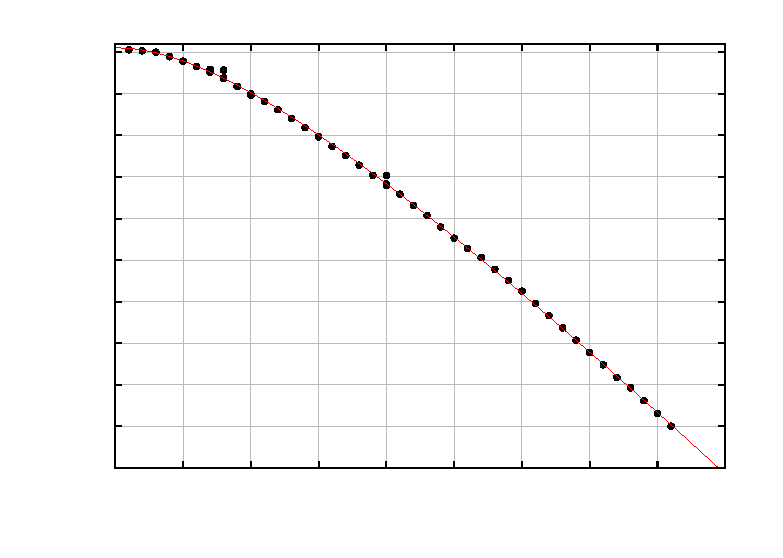
\includegraphics{percent}}%
    \gplfronttext
  \end{picture}%
\endgroup
}
	\end{center}
	\end{figure}
\end{frame}

% =======================================================================
\subsection{Outlook}
\begin{frame}
	\frametitle{Future Goals} 
	\begin{itemize}
		\item Parallelization
		\begin{itemize}
			\item Decrease assignment time
			\item Allow for larger data sets
		\end{itemize}
		\item Machine learning 
		\begin{itemize}
			\item Optimize cost calculation
			\item Increase accuracy of assignment
		\end{itemize}
	\end{itemize} 
\end{frame}

\begin{frame}
	\frametitle{Acknowledgments}
	\begin{itemize}
		\item Dr. Tim Urness (Mathematics and Computer Science)
		\item Dr. Adina Kilpatrick (Physics)
		\item Rachel Davis (research colleague)
		\item John Emmons (research colleague)
		\item  Katherine Roth (research colleague)
		\item  David Mascharka (research colleague)
		\item  Leah Robison (research colleague)
	\end{itemize}
\end{frame}

\begin{frame}{Bibliography}
\nocite{*}
\bibliographystyle{amc}
\bibliography{presentation}
\end{frame}

\begin{frame}
	\frametitle{Thank You} 
	\begin{center}
	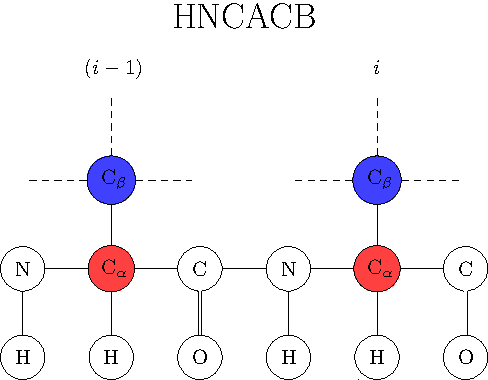
\includegraphics[width=0.3\textwidth]{diagram}\hspace{2em}
	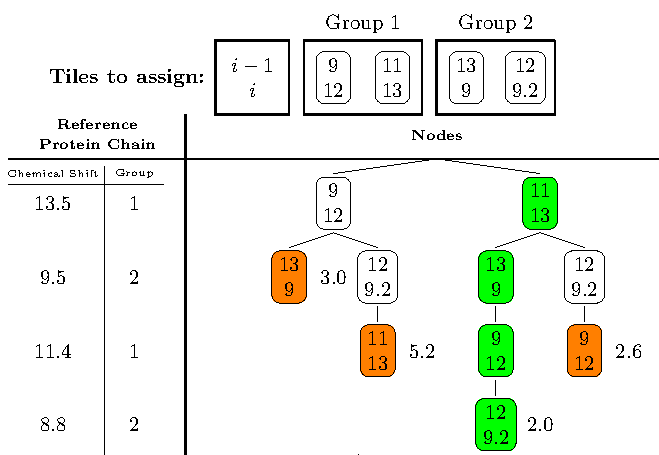
\includegraphics[width=0.4\textwidth]{tilePlacement/step10}
	\end{center}
	\begin{center}
	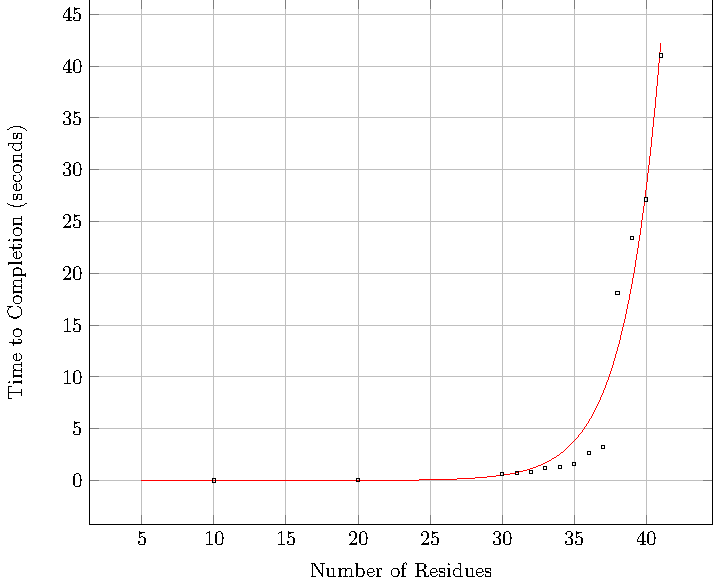
\includegraphics[width=0.3\textwidth]{plot}\hspace{2em}
	\resizebox{!}{.3\paperheight}{% GNUPLOT: LaTeX picture with Postscript
\begingroup
  \makeatletter
  \providecommand\color[2][]{%
    \GenericError{(gnuplot) \space\space\space\@spaces}{%
      Package color not loaded in conjunction with
      terminal option `colourtext'%
    }{See the gnuplot documentation for explanation.%
    }{Either use 'blacktext' in gnuplot or load the package
      color.sty in LaTeX.}%
    \renewcommand\color[2][]{}%
  }%
  \providecommand\includegraphics[2][]{%
    \GenericError{(gnuplot) \space\space\space\@spaces}{%
      Package graphicx or graphics not loaded%
    }{See the gnuplot documentation for explanation.%
    }{The gnuplot epslatex terminal needs graphicx.sty or graphics.sty.}%
    \renewcommand\includegraphics[2][]{}%
  }%
  \providecommand\rotatebox[2]{#2}%
  \@ifundefined{ifGPcolor}{%
    \newif\ifGPcolor
    \GPcolortrue
  }{}%
  \@ifundefined{ifGPblacktext}{%
    \newif\ifGPblacktext
    \GPblacktextfalse
  }{}%
  % define a \g@addto@macro without @ in the name:
  \let\gplgaddtomacro\g@addto@macro
  % define empty templates for all commands taking text:
  \gdef\gplbacktext{}%
  \gdef\gplfronttext{}%
  \makeatother
  \ifGPblacktext
    % no textcolor at all
    \def\colorrgb#1{}%
    \def\colorgray#1{}%
  \else
    % gray or color?
    \ifGPcolor
      \def\colorrgb#1{\color[rgb]{#1}}%
      \def\colorgray#1{\color[gray]{#1}}%
      \expandafter\def\csname LTw\endcsname{\color{white}}%
      \expandafter\def\csname LTb\endcsname{\color{black}}%
      \expandafter\def\csname LTa\endcsname{\color{black}}%
      \expandafter\def\csname LT0\endcsname{\color[rgb]{1,0,0}}%
      \expandafter\def\csname LT1\endcsname{\color[rgb]{0,1,0}}%
      \expandafter\def\csname LT2\endcsname{\color[rgb]{0,0,1}}%
      \expandafter\def\csname LT3\endcsname{\color[rgb]{1,0,1}}%
      \expandafter\def\csname LT4\endcsname{\color[rgb]{0,1,1}}%
      \expandafter\def\csname LT5\endcsname{\color[rgb]{1,1,0}}%
      \expandafter\def\csname LT6\endcsname{\color[rgb]{0,0,0}}%
      \expandafter\def\csname LT7\endcsname{\color[rgb]{1,0.3,0}}%
      \expandafter\def\csname LT8\endcsname{\color[rgb]{0.5,0.5,0.5}}%
    \else
      % gray
      \def\colorrgb#1{\color{black}}%
      \def\colorgray#1{\color[gray]{#1}}%
      \expandafter\def\csname LTw\endcsname{\color{white}}%
      \expandafter\def\csname LTb\endcsname{\color{black}}%
      \expandafter\def\csname LTa\endcsname{\color{black}}%
      \expandafter\def\csname LT0\endcsname{\color{black}}%
      \expandafter\def\csname LT1\endcsname{\color{black}}%
      \expandafter\def\csname LT2\endcsname{\color{black}}%
      \expandafter\def\csname LT3\endcsname{\color{black}}%
      \expandafter\def\csname LT4\endcsname{\color{black}}%
      \expandafter\def\csname LT5\endcsname{\color{black}}%
      \expandafter\def\csname LT6\endcsname{\color{black}}%
      \expandafter\def\csname LT7\endcsname{\color{black}}%
      \expandafter\def\csname LT8\endcsname{\color{black}}%
    \fi
  \fi
  \setlength{\unitlength}{0.0500bp}%
  \begin{picture}(8640.00,6480.00)%
    \gplgaddtomacro\gplbacktext{%
      \csname LTb\endcsname%
      \put(814,704){\makebox(0,0)[r]{\strut{}-45}}%
      \put(814,1303){\makebox(0,0)[r]{\strut{}-40}}%
      \put(814,1902){\makebox(0,0)[r]{\strut{}-35}}%
      \put(814,2501){\makebox(0,0)[r]{\strut{}-30}}%
      \put(814,3100){\makebox(0,0)[r]{\strut{}-25}}%
      \put(814,3699){\makebox(0,0)[r]{\strut{}-20}}%
      \put(814,4298){\makebox(0,0)[r]{\strut{}-15}}%
      \put(814,4897){\makebox(0,0)[r]{\strut{}-10}}%
      \put(814,5496){\makebox(0,0)[r]{\strut{}-5}}%
      \put(814,6095){\makebox(0,0)[r]{\strut{} 0}}%
      \put(946,484){\makebox(0,0){\strut{} 0}}%
      \put(1836,484){\makebox(0,0){\strut{} 5}}%
      \put(2726,484){\makebox(0,0){\strut{} 10}}%
      \put(3616,484){\makebox(0,0){\strut{} 15}}%
      \put(4506,484){\makebox(0,0){\strut{} 20}}%
      \put(5395,484){\makebox(0,0){\strut{} 25}}%
      \put(6285,484){\makebox(0,0){\strut{} 30}}%
      \put(7175,484){\makebox(0,0){\strut{} 35}}%
      \put(8065,484){\makebox(0,0){\strut{} 40}}%
      \put(176,3459){\rotatebox{-270}{\makebox(0,0){\strut{}Percent of possible combinations georated (log(\%))}}}%
      \put(4594,154){\makebox(0,0){\strut{}Number of Amino Acids}}%
    }%
    \gplgaddtomacro\gplfronttext{%
      \csname LTb\endcsname%
      \put(7256,6042){\makebox(0,0)[r]{\strut{}Data}}%
      \csname LTb\endcsname%
      \put(7256,5822){\makebox(0,0)[r]{\strut{}g(x)}}%
    }%
    \gplbacktext
    \put(0,0){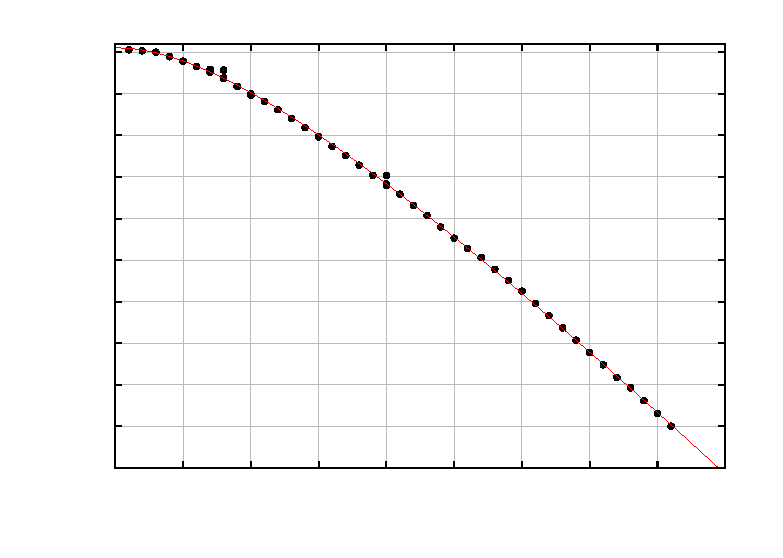
\includegraphics{percent}}%
    \gplfronttext
  \end{picture}%
\endgroup
}
\end{center}
\end{frame}

\end{document}